\documentclass[10pt,a4paper]{article}

% ─── Packages ─────────────────────────────────────────

\usepackage{fontspec}
\setmainfont{Times New Roman}

\usepackage[top=0.6cm,bottom=0.5cm,left=1.45cm,right=1.45cm]{geometry}

\usepackage{titlesec}
\usepackage{enumitem}
\usepackage{hyperref}
\usepackage{xcolor}
\usepackage{tabularx}
\usepackage{graphicx}
\usepackage{parskip}

% ─── Colors ───────────────────────────────────────────

\definecolor{primary}{RGB}{30,40,90}
\definecolor{namecolor}{RGB}{0,120,180}
\definecolor{accent}{RGB}{50,90,150}
\definecolor{rulecol}{RGB}{200,205,220}
\definecolor{gray}{RGB}{90,90,90}

\hypersetup{
    colorlinks=true,
    urlcolor=accent
}

\pagestyle{empty}
\setlength{\parskip}{0pt}

% ─── Section ──────────────────────────────────────────

\titleformat{\section}
    {\normalsize\bfseries\color{primary}}
    {}
    {0em}
    {}
    [\vspace{1pt}\textcolor{rulecol}{\titlerule[0.6pt]}\vspace{1pt}]

\titlespacing{\section}{0pt}{3pt}{1pt}

% ─── Entry ────────────────────────────────────────────

\newcommand{\entry}[3]{%
    \noindent
    \begin{tabularx}{\linewidth}{X r}
        \textbf{\color{primary}#1} &
        {\scriptsize\color{gray}#2}
    \end{tabularx}\\[-2pt]
    {\scriptsize\textit{\color{gray}#3}}
    \vspace{0.5pt}
}

% ─── Compact list ─────────────────────────────────────

\newenvironment{cvitems}{
    \begin{itemize}[
        leftmargin=1.1em,
        topsep=0pt,
        itemsep=0.3pt,
        parsep=0pt,
        partopsep=0pt
    ]
}{
    \end{itemize}
}

% ═════════════════════════════════════════════════════

\begin{document}

% ─── HEADER ───────────────────────────────────────────

\noindent

\begin{tabularx}{\linewidth}{@{}X r@{}}

\begin{minipage}[c]{\linewidth}

    {\LARGE\bfseries\color{namecolor} Hồ Huỳnh Nhu}\\[1pt]

    {\large\bfseries\color{primary}
    Thực tập sinh Phân tích Nghiệp vụ }\\[2pt]

    {\scriptsize\color{gray}
    20/10/2003
    \enspace\textcolor{rulecol}{|}
    \enspace (+84) 367 503 477
    \enspace\textcolor{rulecol}{|}
    \enspace
    \href{mailto:hhnhu2003@gmail.com}{hhnhu2003@gmail.com}
    \enspace\textcolor{rulecol}{|}
    \enspace TP. Hồ Chí Minh}\\[1pt]

    {\scriptsize
    \href{https://github.com/hohuynhnhu}
    {github.com/hohuynhnhu}
    \enspace\textcolor{rulecol}{|}
    \enspace
    \href{https://www.facebook.com/huynhnhu.ho.961}
    {facebook.com/huynhnhu.ho.961}
    }

\end{minipage}

&

\begin{minipage}[c]{2.1cm}
    \raggedleft
    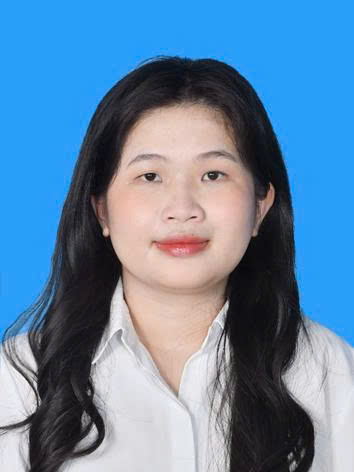
\includegraphics[
        width=2.1cm,
        height=2.5cm,
        keepaspectratio
    ]{assets/avt.jpg}
\end{minipage}

\end{tabularx}

\vspace{1pt}

\textcolor{rulecol}{\rule{\linewidth}{0.6pt}}

% ─── CAREER OBJECTIVE ─────────────────────────────────

\section*{Mục tiêu nghề nghiệp}

{\small
Sinh viên năm cuối ngành Công nghệ Thông tin, có kinh nghiệm thực tế
với SQL, Excel, phân tích dữ liệu và Power BI, cùng với kinh nghiệm
thu thập yêu cầu, làm sạch dữ liệu và xây dựng báo cáo phục vụ ra
quyết định kinh doanh. Có khả năng làm việc với các bên liên quan để
hiểu quy trình và chuyển hóa dữ liệu thành thông tin hữu ích. Mong
muốn ứng tuyển vị trí thực tập Phân tích Nghiệp vụ để phát triển kỹ
năng phân tích quy trình kinh doanh và nền tảng Microsoft Power
Platform (Power Apps, Power Automate, Dataverse).
}

% ─── EDUCATION ────────────────────────────────────────

\section*{Học vấn}

\entry
{Trường Đại học Giao thông Vận tải TP.HCM (UTH)}
{10/2022 -- 10/2026}
{Cử nhân Công nghệ Thông tin -- Đã hoàn thành chương trình học}

{\small
\begin{cvitems}

    \item GPA: \textbf{3.4 / 4.0}

    \item \textbf{Học bổng Xuất sắc} -- Học kỳ 1, 2025

    \item \textbf{Giải Nhì -- Hướng AI},
    Hội nghị Nghiên cứu Khoa học Sinh viên UTH 2025

\end{cvitems}
}

% ─── TECHNICAL SKILLS ─────────────────────────────────

\section*{Kỹ năng}

{\small

\begin{tabularx}{\linewidth}{@{}lX@{}}

\textbf{Phân tích nghiệp vụ}
&
Thu thập yêu cầu, Giao tiếp với các bên liên quan, Phân tích quy
trình As-Is/To-Be, Lập tài liệu quy trình, Xác định KPI, Hỗ trợ UAT
\\[1pt]

\textbf{Dữ liệu \& Báo cáo}
&
Làm sạch dữ liệu, Chuyển đổi dữ liệu, Kiểm tra dữ liệu, Phân tích dữ
liệu khám phá (EDA), Phân tích xu hướng, Báo cáo vận hành
\\[1pt]

\textbf{SQL}
&
SQL, PostgreSQL, SQL Server, MySQL, Joins, CTEs, Aggregations,
Subqueries, Window Functions
\\[1pt]

\textbf{BI / Trực quan hóa}
&
Power BI, DAX, Xây dựng Dashboard, Trực quan hóa dữ liệu
\\[1pt]

\textbf{Excel}
&
Làm sạch dữ liệu, Lọc dữ liệu, Pivot Table, Hàm tra cứu, Báo cáo
\\[1pt]

\textbf{Python}
&
Python, Pandas, NumPy, Tự động hóa xử lý dữ liệu
\\[1pt]

\textbf{ETL / Dữ liệu}
&
ETL/ELT, dbt, Apache Airflow, Data Pipeline, Mô hình hóa dữ liệu
\\[1pt]

\textbf{Cơ sở dữ liệu}
&
PostgreSQL, SQL Server, MySQL, MongoDB, Firebase, Supabase
\\[1pt]

\textbf{Công cụ}
&
Git, Docker, Postman, VS Code, Jira, Confluence
\\[1pt]

\textbf{Đang tự học}
&
Kiến thức nền tảng Power Platform (Power Apps, Power Automate, Dataverse)

\end{tabularx}

}

% ─── WORK EXPERIENCE ──────────────────────────────────

\section*{Kinh nghiệm làm việc}

\entry
{Gotik Consulting -- Data Engineer}
{Python \textbar{} dbt \textbar{} PostgreSQL \textbar{} Airflow \textbar{} Power BI}
{03/2026 -- 05/2026}

{\small
\begin{cvitems}
    \item Làm việc với chủ sở hữu dữ liệu để hiểu quy trình nghiệp vụ
    Odoo và yêu cầu liên quan, sau đó lập tài liệu và chuyển hóa
    thành các tập dữ liệu sạch, có cấu trúc phục vụ phân tích và báo
    cáo.

    \item Xây dựng pipeline ETL bằng Python và mô hình dbt để trích
    xuất, làm sạch và cấu trúc dữ liệu thô thành các tập dữ liệu phân
    tích có thể tái sử dụng trên Neon PostgreSQL, tự động hóa quy
    trình theo giờ bằng Apache Airflow.

    \item Thu thập yêu cầu báo cáo và KPI từ các bên liên quan, xây
    dựng dashboard Power BI hỗ trợ theo dõi và ra quyết định dựa trên
    dữ liệu.

    \item Viết truy vấn SQL để tổng hợp, lọc và kết hợp dữ liệu, đảm
    bảo nguồn dữ liệu đáng tin cậy cho các báo cáo downstream.
\end{cvitems}
}

% ─── PROJECTS ─────────────────────────────────────────

\section*{Dự án tiêu biểu}

\entry
{Delivery Driver -- Hệ thống Phân tích Đơn hàng}
{Python \textbar{} SQL \textbar{} Kafka \textbar{} PostgreSQL \textbar{} Power BI}
{12/2025 -- 02/2026}

{\small
\begin{cvitems}
    \item Thu thập và phân tích yêu cầu báo cáo dữ liệu đơn hàng; xây
    dựng pipeline Data Lake / Data Warehouse để chuẩn bị dữ liệu cho
    phân tích.
    \item Áp dụng RFM và Association Rule Mining để phân tích hành vi
    khách hàng và phát hiện các mẫu hình lấy--giao hàng thường gặp
    phục vụ mục đích kinh doanh.
    \item GitHub: \href{https://github.com/LeKhang-cn22h/BE-delivery-driver}{BE-delivery-driver}
\end{cvitems}
}

\vspace{1pt}

\entry
{VehicleScan -- Hệ thống Dữ liệu Bãi đỗ xe Thông minh}
{Python \textbar{} SQL \textbar{} PostgreSQL \textbar{} Firebase \textbar{} ESP32}
{03/2025 -- 03/2026}

{\small
\begin{cvitems}
    \item Phân tích yêu cầu vận hành cho bài toán giám sát bãi đỗ xe
    thời gian thực, xử lý dữ liệu xe và cảm biến IoT bằng Python và
    SQL.
    \item Tích hợp dữ liệu AI, cảm biến và ứng dụng vào một hệ thống
    tập trung để hỗ trợ giám sát và báo cáo.
    \item GitHub: \href{https://github.com/LeKhang-cn22h/VehicleScanner}{VehicleScanner}
\end{cvitems}
}

% ─── ADDITIONAL INFORMATION ───────────────────────────

\section*{Thông tin thêm}

{\small

\begin{tabularx}{\linewidth}{@{}lX@{}}

\textbf{Tiếng Anh}
&
Đọc hiểu tài liệu kỹ thuật và giao tiếp chuyên môn cơ bản

\\[1pt]

\textbf{Tình trạng}
&
Sẵn sàng thực tập toàn thời gian hoặc bán thời gian vị trí Phân tích
Nghiệp vụ

\end{tabularx}

}
\end{document}